\documentclass[class=report,crop=false, 12pt]{standalone}
\usepackage[screen,nosolutions]{../myscratch}
%\usepackage[screen]{../myscratch}



\begin{document}

\titre[S]{Sons}
%===============================

\insertvideo{_mubpJPmHsk}{Sons -- Activité 1}

\insertvideo{X5uMtGK1wrw}{Sons -- Activité 2}

\insertvideo{mndn-wTrOjE}{Sons -- Activité 3}

\bigskip
\bigskip

\emph{Scratch permet de jouer des sons, des notes avec divers instruments, et même d'enregistrer ses propres sons. On va ici s'intéresser plutôt à l'aspect scientifique du son.}

\bigskip
\bigskip



\begin{activite}

\sauteligne

\begin{center}
  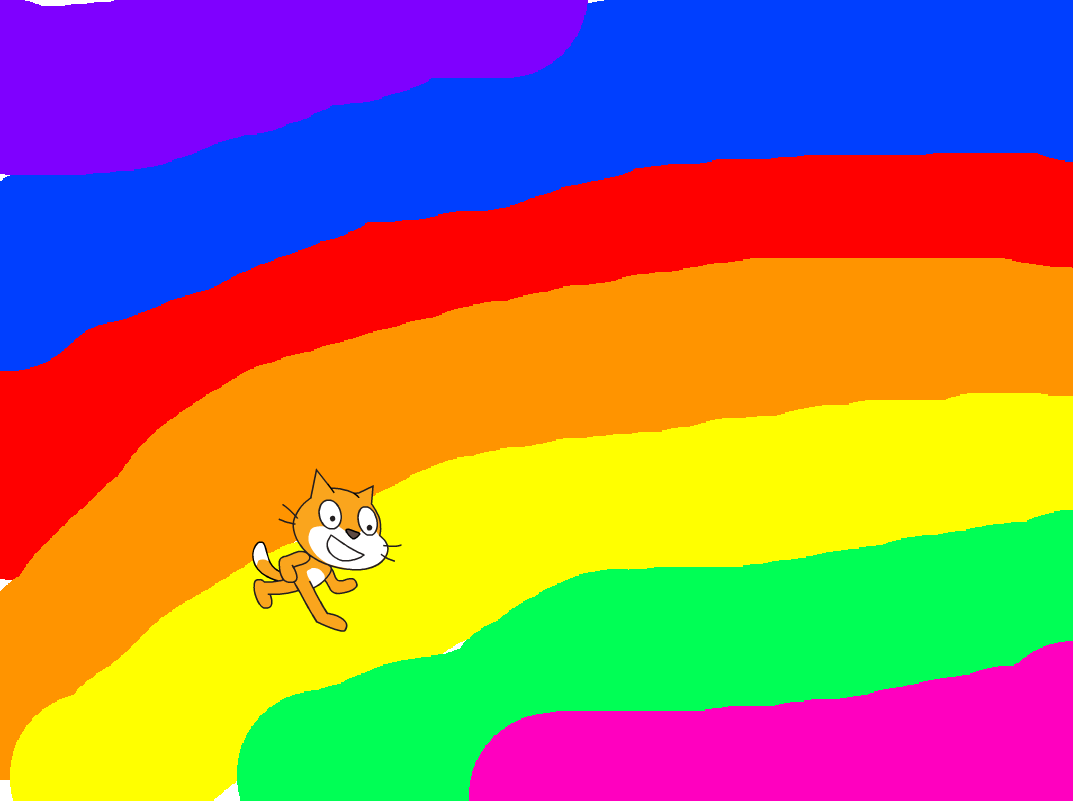
\includegraphics[width=0.6\textwidth]{ecran-09-ex1} 
\end{center}

Scratch se déplace sur un arc-en-ciel et joue une musique en fonction de la couleur sur laquelle il se trouve.

\begin{enumerate}
  \item Dessine un arrière-plan avec plusieurs couleurs différentes.
  \item Fais déplacer Scratch sur tout l'écran.
  \item Joue une note \emph{do}, \emph{ré}, \emph{mi}... selon la couleur. 
  \item Tu peux choisir un nombre au hasard pour la durée du son  
  (par exemple $0.05$ fois un nombre aléatoire entre $1$ et $10$). 
\end{enumerate}

\medskip

\textbf{Blocs utiles.}

Afin de permettre à Scratch de jouer des sons, ajoute l'extension \og{}Musique\fg{}. 
Les notes sont énumérées à l'aide d'entiers, \emph{do} est représenté par $60$, 
%(emprunté à la numérotation MIDI),
\emph{ré} par $62$\ldots{} On y accède à l'aide d'une image représentant les touches d'un piano.


%% \begin{center}
%%   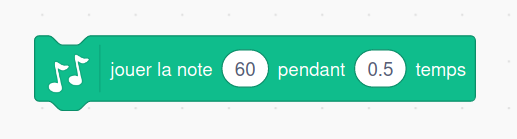
\includegraphics[width=0.4\textwidth]{bloc-music} 
%% \end{center}

\begin{center}
\begin{scratch}
  \blockmusic{jouer la note \ovalnum{60} pendant \ovalnum{0.5} temps}
\end{scratch}
\end{center}


\end{activite}



\begin{activite}[Le son est une onde]

\sauteligne

\begin{center}
  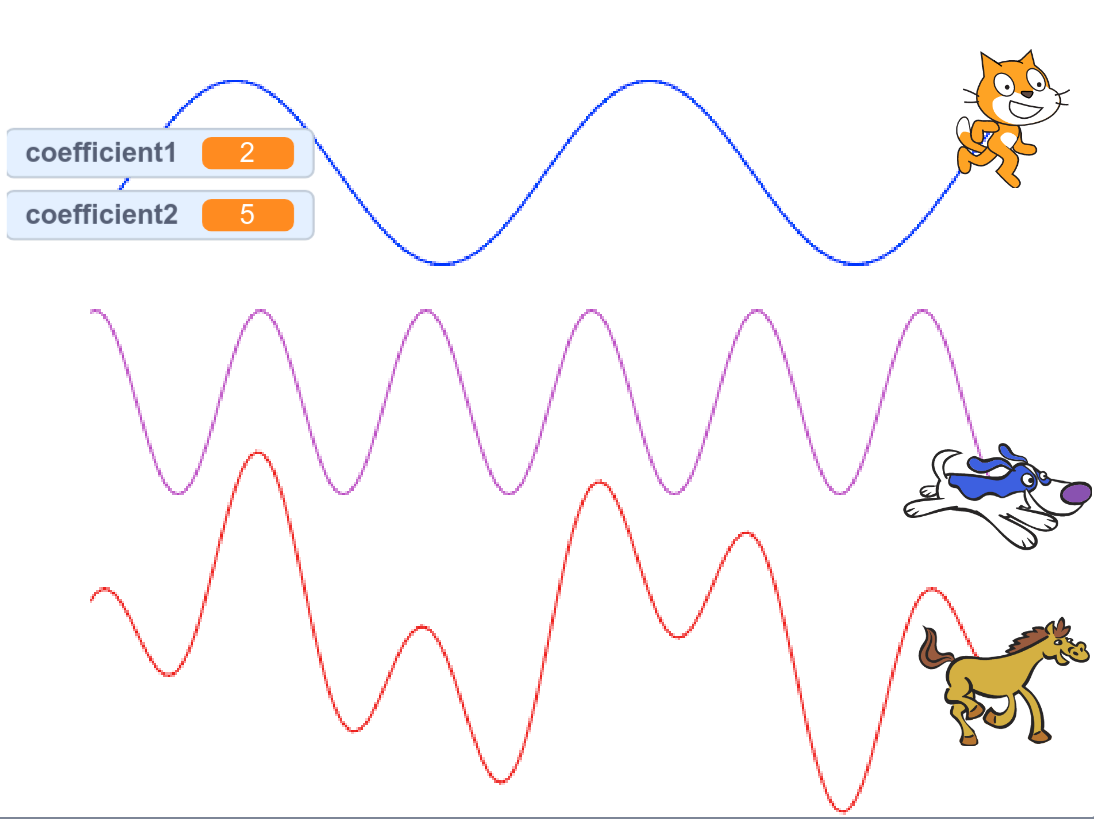
\includegraphics[width=0.6\textwidth]{ecran-09-ex2} 
\end{center}

\begin{itemize}
  \item Le son se propage en faisant vibrer l'air : on parle d'une onde. 
  \item C'est comme lorsque l'on jette un caillou dans l'eau, des vagues se forment.
  \item Ces vagues seront ici des \emph{sinus}. Les sommets des vagues sont plus ou moins rapprochés selon la \emph{fréquence}.
\end{itemize} 


\myfigure{1}{
\tikzinput{onde}
} 
\begin{enumerate}
  \item Partir de $x=-200$.
  
  \item Calculer :
  \begin{itemize}
    \item Mettre la variable \codeinline{y1} selon la formule : $y_1 = 40 \times \sin(2 \times x)$.
    \item Mettre la variable \codeinline{y2} selon la formule : $y_2 = 40 \times \sin(5 \times x)$.  
    \item Mettre la variable  \codeinline{y3} selon la formule : $y_3 = y_1+y_2$.    
  \end{itemize}
  
  \item Le chat va à $(x,y_1+100)$, le chien à $(x,y_2)$, le cheval à $(x,y_3-100)$.
  
  \item Recommencer après avoir augmenté la valeur de $x$.
  
  \item \textbf{Bonus.} Définir deux variables \codeinline{coeff1} et \codeinline{coeff2} qui permettent de changer les fréquences :
  $$y_1 = 40 \times \sin(\text{\codeinline{coeff1}} \times x)
  \qquad y_2 = 40 \times \sin(\text{\codeinline{coeff2}} \times x)$$ 
  
\end{enumerate}  

\medskip
\textbf{Blocs utiles.}

Dans la catégorie \og Opérateur \fg{}, tout en bas, tu trouveras les fonctions mathématiques, dont la fonction \og sinus\fg{}.

\begin{center}
  \ovaloperator{\selectmenu{sin} de \ovalvariable{nombre}}
\end{center}

\end{activite}



\begin{activite}[L'effet Doppler]

Tu entends l'\emph{effet Doppler} avec la sirène des pompiers : quand la sirène se rapproche le son devient plus aigu, quand la sirène s'éloigne le son devient plus grave.
La sirène des pompiers émet toujours le même son, à la même fréquence, mais celui-ci est perçu différemment. 

\myfigure{0.40}{
\tikzinput{doppler1}\quad
\tikzinput{doppler2}
} 

Sur la figure de gauche le camion est fixe, sur celle de droite il se déplace.
Pour modéliser le son, on imagine que la sirène émet un \og bip \fg{} à chaque seconde.
Le son se propage et on représente ce \og bip \fg{} par un cercle qui part de la sirène puis s'agrandit.

\begin{center}
  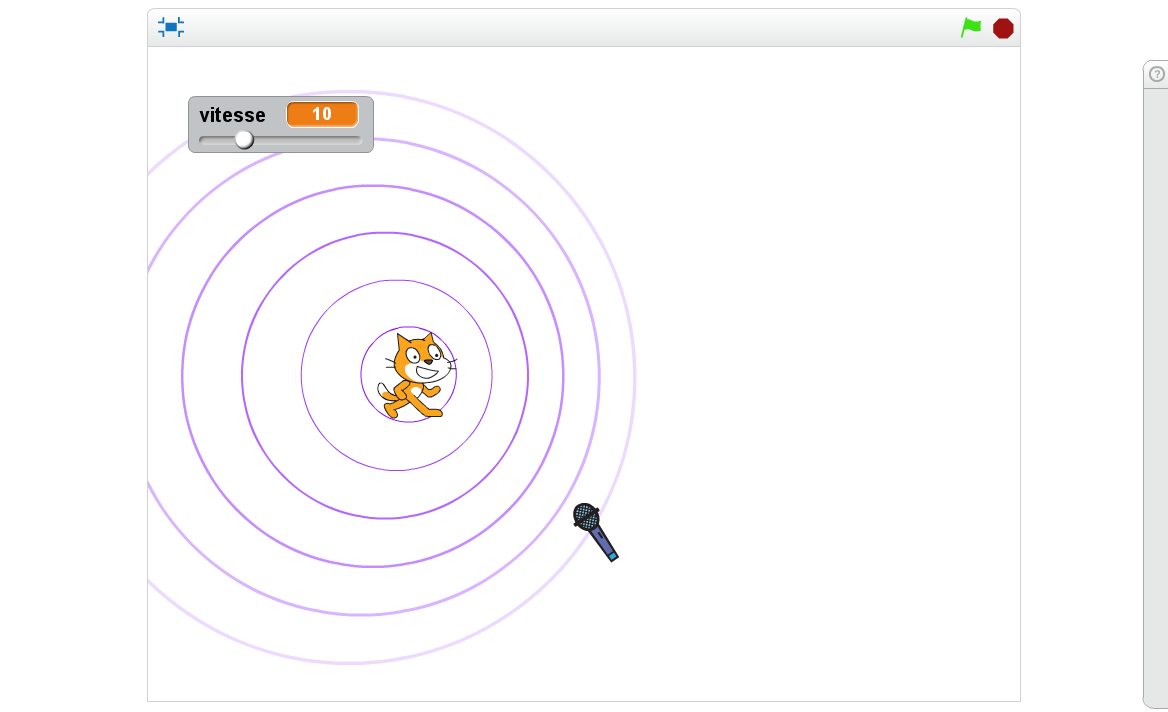
\includegraphics[width=0.8\textwidth]{ecran-09-ex3} 
\end{center}


\bigskip

\textbf{Le chat.}

Le chat représente le camion de pompier.
Définis une variable \codeinline{vitesse}, puis répète indéfiniment :

\begin{enumerate}
  \item avancer de \codeinline{vitesse},
  \item attendre $1$ seconde,
  \item créer un clone du lutin \og Cercle \fg{}.
\end{enumerate}

\bigskip

\textbf{Les cercles.}

Dessine toi-même le lutin \og Cercle \fg{} : c'est juste un grand cercle. 
Il sera cloné plusieurs fois et sera affiché à des tailles différentes.

Quand le lutin \og{}Cercle\fg{} démarre comme un clone :
\begin{enumerate}
  \item il se place là où est le chat,
  \item il s'affiche avec un taille de $0\%$,
  \item puis répète $20$ fois : attendre $0.3$ seconde, ajouter $5$ à la taille.
  \item Tu peux utiliser l'effet \og fantôme \fg{} pour estomper progressivement le cercle.
\end{enumerate}


\bigskip
\textbf{Bonus. Le microphone.}

\begin{itemize}
  \item Si un cercle touche le microphone, alors joue un son bref.
  \item Attention : le microphone doit être mis à une taille très petite, afin de ne toucher chaque cercle qu'une seule fois.
\end{itemize}




\bigskip
\textbf{Utilisation.}

\begin{itemize}
  \item À vitesse nulle. Les cercles ont tous le même centre. Le microphone joue un son régulièrement.
  
  \item À petite vitesse. Les cercles sont plus regroupés vers l'avant. Le microphone joue des sons d'abord rapprochés, puis plus espacés. 
  
  \item À grande vitesse. Lorsque le chat se déplace à la même vitesse que le son, alors les cercles peuvent avoir tous un point commun : c'est le phénomène du mur du son ! 
\end{itemize}

\end{activite}


\ifx \displaysolutions \myzero
\else
\begin{code}
\setscratch{scale=\scalesolution}
\onesolution{Sons}{Activité 1}{
\begin{scratch}
  \blockinit{quand \greenflag est cliqué}
  \blockinfloop{répéter indéfiniment}
  {
    \blockmove{avancer de \ovalnum{30} pas} 
    \blockmove{tourner \turnright{} de \ovalnum{10} degrés}
    \blockmove{rebondir si le bord est atteint}
    \blockvariable{mettre \selectmenu{duree} à \ovaloperator{\ovalnum{0.05} * \ovaloperator{nombre aléatoire entre \ovalnum{1} et \ovalnum{10}}}}
    \blockif{si \boolsensing{couleur \pencolor{green!70!black} touchée ?} alors }
    {
      \blockmusic{jouer la note \ovalnum{60} pendant \ovalvariable{duree} temps}
    }
    \blockif{si \boolsensing{couleur \pencolor{red!70!black} touchée ?} alors }
    {
      \blockmusic{jouer la note \ovalnum{62} pendant \ovalvariable{duree} temps}
    }
  }
\end{scratch}
}
\onesolution{Sons}{Activité 2}{
\begin{minipage}{0.4\textwidth}
\hbox{Chat} 
\begin{scratch}
  \blockinit{quand \greenflag est cliqué}
  \blockvariable{mettre \selectmenu{coeff1} à \ovalnum{2}}
  \blockvariable{mettre \selectmenu{coeff2} à \ovalnum{5}}
  \blockvariable{mettre \selectmenu{x} à \ovalnum{-200}}
  \blockpen{effacer tout}
  \blockpen{stylo en position d'écriture}
  \blockrepeat{répéter \ovalnum{200} fois}
  {
    \blockvariable{mettre \selectmenu{y1} à \ovaloperator{ \ovalnum{40} *       \ovaloperator{\selectmenu{sin} de \ovaloperator{ \ovalvariable{coeff1} * \ovalvariable{x}}}}}
    \blockvariable{mettre \selectmenu{y2} à \ovaloperator{ \ovalnum{40} *       \ovaloperator{\selectmenu{sin} de \ovaloperator{ \ovalvariable{coeff2} * \ovalvariable{x}}}}}
    \blockvariable{mettre \selectmenu{y3} à \ovaloperator{ \ovalvariable{y1} + \ovalvariable{y2} }}
    \blockmove{aller à x: \ovalvariable{x} y: \ovaloperator{\ovalnum{100} + \ovalvariable{y1}}}
    \blockvariable{ajouter \ovalnum{2} à \selectmenu{x}}
  }
\end{scratch}
%\end{minipage}
%\begin{minipage}{0.35\textwidth}

\medskip

\hbox{Chien (le cheval est semblable)}
\begin{scratch}
  \blockinit{quand \greenflag est cliqué}
  \blockpen{stylo en position d'écriture}
  \blockrepeat{répéter \ovalnum{200} fois}
  {
    \blockmove{aller à x: \ovalvariable{x} y: \ovalvariable{y2}}
  }
\end{scratch}
\end{minipage}
}

\medskip

\onesolution{Sons}{Activité 3}{
\begin{minipage}{0.25\textwidth}
\hbox{Chat} 
\begin{scratch}
  \blockinit{quand \greenflag est cliqué}
  \blockmove{aller à x: \ovalnum{-200} y: \ovalnum{0}}
  \blockpen{effacer tout}
  \blockvariable{mettre \selectmenu{vitesse} à \ovalnum{10}}
  \blockinfloop{répéter indéfiniment}
  {
    \blockmove{avancer de \ovalvariable{vitesse} pas} 
    \blockmove{rebondir si le bord est atteint}
    \blockcontrol{attendre \ovalnum{1} secondes} 
    \blockcontrol{créer un clone de \ovalcontrol*{Cercle}} 
  }
\end{scratch}
\end{minipage}
\begin{minipage}{0.25\textwidth}
\hbox{Cercle}
\begin{scratch}
  \blockinitclone{quand je commence comme un clone}
  \blockcontrol{attendre \ovalnum{1} secondes} 
  \blockmove{aller à \ovalmove*{Chat}}
  \blocklook{mettre la taille à \ovalnum{0}\% de la taille initiale}
  \blocklook{mettre l'effet \selectmenu{fantôme} à \ovalnum{0}}
  \blocklook{montrer}
  \blockrepeat{répéter \ovalnum{20} fois}
  {
    \blockcontrol{attendre \ovalnum{0.3} secondes} 
    \blocklook{ajouter \ovalnum{5} à la taille}
    \blocklook{ajouter \ovalnum{5} à l'effet \selectmenu{fantôme}}
  }
  \blocklook{cacher}
  \blockstop{supprimer ce clone}
\end{scratch}
\end{minipage}
\begin{minipage}{0.25\textwidth}
\hbox{Microphone}
\begin{scratch}
  \blockinit{quand \greenflag est cliqué}
  \blocklook{mettre la taille à \ovalnum{100}\% de la taille initiale}
  \blockrepeat{répéter \ovalnum{10} fois}
  {
    \blocklook{ajouter \ovalnum{-10} à la taille}
    \blockcontrol{attendre \ovalnum{0.5} secondes} 
  }
  \blockinfloop{répéter indéfiniment}
  {
    \blockif{si \boolsensing{touche le \ovalsensing*{Cercle} ?} alors }
    {
      \blockmusic{jouer la note \ovalnum{60} pendant \ovalnum{0.3} temps}
    }
  }
\end{scratch}
\end{minipage}
}
\end{code}
\fi

\end{document}
